% Created by tikzDevice version 0.10.1 on 2017-11-13 11:16:29
% !TEX encoding = UTF-8 Unicode
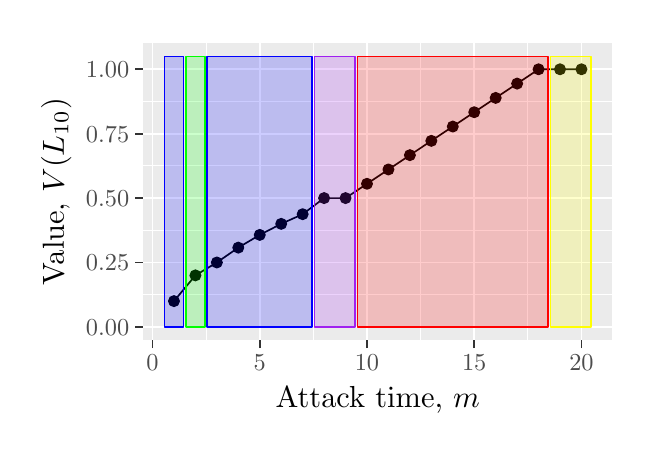
\begin{tikzpicture}[x=1pt,y=1pt]
\definecolor{fillColor}{RGB}{255,255,255}
\path[use as bounding box,fill=fillColor,fill opacity=0.00] (0,0) rectangle (216.81,144.54);
\begin{scope}
\path[clip] (  0.00,  0.00) rectangle (216.81,144.54);
\definecolor{drawColor}{RGB}{255,255,255}
\definecolor{fillColor}{RGB}{255,255,255}

\path[draw=drawColor,line width= 0.6pt,line join=round,line cap=round,fill=fillColor] (  0.00,  0.00) rectangle (216.81,144.54);
\end{scope}
\begin{scope}
\path[clip] ( 41.67, 31.53) rectangle (211.31,139.04);
\definecolor{fillColor}{gray}{0.92}

\path[fill=fillColor] ( 41.67, 31.53) rectangle (211.31,139.04);
\definecolor{drawColor}{RGB}{255,255,255}

\path[draw=drawColor,line width= 0.3pt,line join=round] ( 41.67, 48.05) --
	(211.31, 48.05);

\path[draw=drawColor,line width= 0.3pt,line join=round] ( 41.67, 71.32) --
	(211.31, 71.32);

\path[draw=drawColor,line width= 0.3pt,line join=round] ( 41.67, 94.59) --
	(211.31, 94.59);

\path[draw=drawColor,line width= 0.3pt,line join=round] ( 41.67,117.86) --
	(211.31,117.86);

\path[draw=drawColor,line width= 0.3pt,line join=round] ( 64.49, 31.53) --
	( 64.49,139.04);

\path[draw=drawColor,line width= 0.3pt,line join=round] (103.24, 31.53) --
	(103.24,139.04);

\path[draw=drawColor,line width= 0.3pt,line join=round] (141.99, 31.53) --
	(141.99,139.04);

\path[draw=drawColor,line width= 0.3pt,line join=round] (180.74, 31.53) --
	(180.74,139.04);

\path[draw=drawColor,line width= 0.6pt,line join=round] ( 41.67, 36.42) --
	(211.31, 36.42);

\path[draw=drawColor,line width= 0.6pt,line join=round] ( 41.67, 59.69) --
	(211.31, 59.69);

\path[draw=drawColor,line width= 0.6pt,line join=round] ( 41.67, 82.96) --
	(211.31, 82.96);

\path[draw=drawColor,line width= 0.6pt,line join=round] ( 41.67,106.23) --
	(211.31,106.23);

\path[draw=drawColor,line width= 0.6pt,line join=round] ( 41.67,129.50) --
	(211.31,129.50);

\path[draw=drawColor,line width= 0.6pt,line join=round] ( 45.11, 31.53) --
	( 45.11,139.04);

\path[draw=drawColor,line width= 0.6pt,line join=round] ( 83.86, 31.53) --
	( 83.86,139.04);

\path[draw=drawColor,line width= 0.6pt,line join=round] (122.61, 31.53) --
	(122.61,139.04);

\path[draw=drawColor,line width= 0.6pt,line join=round] (161.36, 31.53) --
	(161.36,139.04);

\path[draw=drawColor,line width= 0.6pt,line join=round] (200.11, 31.53) --
	(200.11,139.04);
\definecolor{drawColor}{RGB}{0,0,0}
\definecolor{fillColor}{RGB}{0,0,0}

\path[draw=drawColor,line width= 0.4pt,line join=round,line cap=round,fill=fillColor] (192.36,129.50) circle (  1.96);

\path[draw=drawColor,line width= 0.4pt,line join=round,line cap=round,fill=fillColor] (200.11,129.50) circle (  1.96);

\path[draw=drawColor,line width= 0.4pt,line join=round,line cap=round,fill=fillColor] (122.61, 88.13) circle (  1.96);

\path[draw=drawColor,line width= 0.4pt,line join=round,line cap=round,fill=fillColor] (130.36, 93.30) circle (  1.96);

\path[draw=drawColor,line width= 0.4pt,line join=round,line cap=round,fill=fillColor] (138.11, 98.47) circle (  1.96);

\path[draw=drawColor,line width= 0.4pt,line join=round,line cap=round,fill=fillColor] (145.86,103.64) circle (  1.96);

\path[draw=drawColor,line width= 0.4pt,line join=round,line cap=round,fill=fillColor] (153.61,108.81) circle (  1.96);

\path[draw=drawColor,line width= 0.4pt,line join=round,line cap=round,fill=fillColor] (161.36,113.99) circle (  1.96);

\path[draw=drawColor,line width= 0.4pt,line join=round,line cap=round,fill=fillColor] (169.11,119.16) circle (  1.96);

\path[draw=drawColor,line width= 0.4pt,line join=round,line cap=round,fill=fillColor] (176.86,124.33) circle (  1.96);

\path[draw=drawColor,line width= 0.4pt,line join=round,line cap=round,fill=fillColor] (184.61,129.50) circle (  1.96);

\path[draw=drawColor,line width= 0.4pt,line join=round,line cap=round,fill=fillColor] ( 60.61, 55.03) circle (  1.96);

\path[draw=drawColor,line width= 0.4pt,line join=round,line cap=round,fill=fillColor] (114.86, 82.96) circle (  1.96);

\path[draw=drawColor,line width= 0.4pt,line join=round,line cap=round,fill=fillColor] (107.11, 82.96) circle (  1.96);

\path[draw=drawColor,line width= 0.4pt,line join=round,line cap=round,fill=fillColor] ( 68.36, 59.69) circle (  1.96);

\path[draw=drawColor,line width= 0.4pt,line join=round,line cap=round,fill=fillColor] ( 76.11, 65.06) circle (  1.96);

\path[draw=drawColor,line width= 0.4pt,line join=round,line cap=round,fill=fillColor] ( 83.86, 69.66) circle (  1.96);

\path[draw=drawColor,line width= 0.4pt,line join=round,line cap=round,fill=fillColor] ( 91.61, 73.65) circle (  1.96);

\path[draw=drawColor,line width= 0.4pt,line join=round,line cap=round,fill=fillColor] ( 99.36, 77.14) circle (  1.96);

\path[draw=drawColor,line width= 0.4pt,line join=round,line cap=round,fill=fillColor] ( 52.86, 45.73) circle (  1.96);

\path[draw=drawColor,line width= 0.6pt,line join=round] ( 52.86, 45.73) --
	( 60.61, 55.03) --
	( 68.36, 59.69) --
	( 76.11, 65.06) --
	( 83.86, 69.66) --
	( 91.61, 73.65) --
	( 99.36, 77.14) --
	(107.11, 82.96) --
	(114.86, 82.96) --
	(122.61, 88.13) --
	(130.36, 93.30) --
	(138.11, 98.47) --
	(145.86,103.64) --
	(153.61,108.81) --
	(161.36,113.99) --
	(169.11,119.16) --
	(176.86,124.33) --
	(184.61,129.50) --
	(192.36,129.50) --
	(200.11,129.50);
\definecolor{drawColor}{RGB}{255,255,0}
\definecolor{fillColor}{RGB}{255,255,0}

\path[draw=drawColor,line width= 0.6pt,line join=round,fill=fillColor,fill opacity=0.20] (188.87, 36.42) rectangle (203.60,134.15);
\definecolor{drawColor}{RGB}{255,0,0}
\definecolor{fillColor}{RGB}{255,0,0}

\path[draw=drawColor,line width= 0.6pt,line join=round,fill=fillColor,fill opacity=0.20] (119.13, 36.42) rectangle (188.10,134.15);
\definecolor{drawColor}{RGB}{160,32,240}
\definecolor{fillColor}{RGB}{160,32,240}

\path[draw=drawColor,line width= 0.6pt,line join=round,fill=fillColor,fill opacity=0.20] (103.63, 36.42) rectangle (118.35,134.15);
\definecolor{drawColor}{RGB}{0,0,255}
\definecolor{fillColor}{RGB}{0,0,255}

\path[draw=drawColor,line width= 0.6pt,line join=round,fill=fillColor,fill opacity=0.20] ( 64.88, 36.42) rectangle (102.85,134.15);
\definecolor{drawColor}{RGB}{0,255,0}
\definecolor{fillColor}{RGB}{0,255,0}

\path[draw=drawColor,line width= 0.6pt,line join=round,fill=fillColor,fill opacity=0.20] ( 57.13, 36.42) rectangle ( 64.10,134.15);
\definecolor{drawColor}{RGB}{0,0,255}
\definecolor{fillColor}{RGB}{0,0,255}

\path[draw=drawColor,line width= 0.6pt,line join=round,fill=fillColor,fill opacity=0.20] ( 49.38, 36.42) rectangle ( 56.35,134.15);
\end{scope}
\begin{scope}
\path[clip] (  0.00,  0.00) rectangle (216.81,144.54);
\definecolor{drawColor}{gray}{0.30}

\node[text=drawColor,anchor=base east,inner sep=0pt, outer sep=0pt, scale=  0.88] at ( 36.72, 33.39) {0.00};

\node[text=drawColor,anchor=base east,inner sep=0pt, outer sep=0pt, scale=  0.88] at ( 36.72, 56.66) {0.25};

\node[text=drawColor,anchor=base east,inner sep=0pt, outer sep=0pt, scale=  0.88] at ( 36.72, 79.93) {0.50};

\node[text=drawColor,anchor=base east,inner sep=0pt, outer sep=0pt, scale=  0.88] at ( 36.72,103.20) {0.75};

\node[text=drawColor,anchor=base east,inner sep=0pt, outer sep=0pt, scale=  0.88] at ( 36.72,126.47) {1.00};
\end{scope}
\begin{scope}
\path[clip] (  0.00,  0.00) rectangle (216.81,144.54);
\definecolor{drawColor}{gray}{0.20}

\path[draw=drawColor,line width= 0.6pt,line join=round] ( 38.92, 36.42) --
	( 41.67, 36.42);

\path[draw=drawColor,line width= 0.6pt,line join=round] ( 38.92, 59.69) --
	( 41.67, 59.69);

\path[draw=drawColor,line width= 0.6pt,line join=round] ( 38.92, 82.96) --
	( 41.67, 82.96);

\path[draw=drawColor,line width= 0.6pt,line join=round] ( 38.92,106.23) --
	( 41.67,106.23);

\path[draw=drawColor,line width= 0.6pt,line join=round] ( 38.92,129.50) --
	( 41.67,129.50);
\end{scope}
\begin{scope}
\path[clip] (  0.00,  0.00) rectangle (216.81,144.54);
\definecolor{drawColor}{gray}{0.20}

\path[draw=drawColor,line width= 0.6pt,line join=round] ( 45.11, 28.78) --
	( 45.11, 31.53);

\path[draw=drawColor,line width= 0.6pt,line join=round] ( 83.86, 28.78) --
	( 83.86, 31.53);

\path[draw=drawColor,line width= 0.6pt,line join=round] (122.61, 28.78) --
	(122.61, 31.53);

\path[draw=drawColor,line width= 0.6pt,line join=round] (161.36, 28.78) --
	(161.36, 31.53);

\path[draw=drawColor,line width= 0.6pt,line join=round] (200.11, 28.78) --
	(200.11, 31.53);
\end{scope}
\begin{scope}
\path[clip] (  0.00,  0.00) rectangle (216.81,144.54);
\definecolor{drawColor}{gray}{0.30}

\node[text=drawColor,anchor=base,inner sep=0pt, outer sep=0pt, scale=  0.88] at ( 45.11, 20.52) {0};

\node[text=drawColor,anchor=base,inner sep=0pt, outer sep=0pt, scale=  0.88] at ( 83.86, 20.52) {5};

\node[text=drawColor,anchor=base,inner sep=0pt, outer sep=0pt, scale=  0.88] at (122.61, 20.52) {10};

\node[text=drawColor,anchor=base,inner sep=0pt, outer sep=0pt, scale=  0.88] at (161.36, 20.52) {15};

\node[text=drawColor,anchor=base,inner sep=0pt, outer sep=0pt, scale=  0.88] at (200.11, 20.52) {20};
\end{scope}
\begin{scope}
\path[clip] (  0.00,  0.00) rectangle (216.81,144.54);
\definecolor{drawColor}{RGB}{0,0,0}

\node[text=drawColor,anchor=base,inner sep=0pt, outer sep=0pt, scale=  1.10] at (126.49,  7.44) {Attack time, $m$};
\end{scope}
\begin{scope}
\path[clip] (  0.00,  0.00) rectangle (216.81,144.54);
\definecolor{drawColor}{RGB}{0,0,0}

\node[text=drawColor,rotate= 90.00,anchor=base,inner sep=0pt, outer sep=0pt, scale=  1.10] at ( 13.08, 85.29) {Value, $V(L_{ 10 })$};
\end{scope}
\end{tikzpicture}
